\documentclass[a4paper, 11pt]{article}
\usepackage{comment} % enables the use of multi-line comments (\ifx \fi) 
\usepackage{fullpage} % changes the margin
\usepackage{xcolor}
\usepackage{listings}
\lstdefinestyle{BashInputStyle}{
  language=bash,
  breaklines=true,
  basicstyle=\smallskip\sffamily,
  numbers=left,
  numberstyle=\tiny,
  numbersep=11pt,
  frame=tb,
  columns=fullflexible,
  backgroundcolor=\color{yellow!15},
  linewidth=0.9\linewidth,
  xleftmargin=0.1\linewidth,
  showstringspaces=false
}
\usepackage{graphics}
\usepackage{graphicx}
\usepackage[colorlinks = true,
            linkcolor = blue,
            urlcolor  = blue,
            citecolor = blue,
            anchorcolor = blue]{hyperref}
\usepackage[toc,page]{appendix}
\usepackage{pgfplots}
\pgfplotsset{compat=1.14}
\graphicspath{ {images/} }

\begin{document}
%Header-Make sure you update this information!!!!
\noindent
\large\textbf{Computer Networks : Lab Assignment 1} \hfill \textbf{Shreshth Tuli} \\
\normalsize COL334 \hfill 2016CS10680 \\
Prof. B.N. Jain \hfill Date: 17/08/2018 \\

This Lab Assignment aims to introduce networking concepts and network topologies.

\section{Part A - Networking tools}

\subsection{Internet access performance analysis}

The experiment performed was to analyze the Download and Upload speeds from different tools. Two tools used were \url{http://www.testmyspeed.com/} and \url{http://www.speedtest.net/}. These tests were performed from the Lecture Hall Complex of IITD. The results from these tools are shown below:

\begin{lstlisting}[style=BashInputStyle]
Testmyspeed.com – 
DL : 68.50 Mb/s , UL : 17.02 Mb/s
Speedtest.net – 
DL : 97.81 Mb/s, UL : 120.83 Mb/s, Ping : 6 ms
\end{lstlisting}

The two results are significantly different from each other. The reasons can be:
\begin{itemize}
\item Fluctuations in the Internet connectivity across different tests
\item Changing network route due to changing servers or hosts to which the system connects to for different tests which changes overall download and upload speeds
\item Different benchmarking and testing procedures used by the two anaylsis tools 
\end{itemize}
 
\subsection{Ping network utility}

\subsubsection{About Ping}

Ping is a network utility that helps to check the reachability of a host on the network which follows Internet Protocol (IP). Ping works by sending Internet Control Message Protocol (ICMP) echo packets to the target host and waits for an ICMP echo reply. It works similar to the Sonar system and reports Round Trip Time (RTT), packet loss, and other statistical measures.

\subsubsection{Experiments with ping}

Ping was used to know the IP addresses and RTT of servers. The experiment was performed on three servers: \url{www.google.com}, \url{www.harvard.edu}, \url{www.iitd.ac.in}. The results are shown below. Full results can be seen in appendix \ref{appendix:ping}.

\begin{lstlisting}[style=BashInputStyle]
ping www.google.com
Pinging www.google.com [216.58.221.36]
Approximate round trip times in milli-seconds:
    Minimum = 5ms, Maximum = 6ms, Average = 5ms
\end{lstlisting}  

\begin{lstlisting}[style=BashInputStyle]
ping www.harvard.edu
Pinging www.harvard.edu.cdn.cloudflare.net [104.16.155.6]
Approximate round trip times in milli-seconds:
    Minimum = 46ms, Maximum = 47ms, Average = 46ms
\end{lstlisting}  

\begin{lstlisting}[style=BashInputStyle]
ping www.iitd.ac.in
Pinging www.iitd.ac.in [10.7.174.111]
Approximate round trip times in milli-seconds:
    Minimum = 2ms, Maximum = 3ms, Average = 2ms
\end{lstlisting}

We can see that the average RTT for the three: google, harvard and iitd are 5ms, 46ms, 2ms. Their IP addresses are: 216.58.221.36, 104.16.155.6 and 10.7.174.111 respectively. In terms of RTT the closest server is 'iitd'. This is clearly because the tests were performed from within IITD network and thus has lesser round trip time. The farthest in terms of RTT is 'harvard' because of distant target server that the system is connecting to (target server being in the US and source server in India). Google on the other hand has several servers across the globe and thus the system connects to the nearest and has much lesser RTT, probably the server is in India itself.

\subsection{'ifconfig' network command}

The 'ifconfig' network command provides information of all the network interfaces of the system. The detailed output of the ifconfig command can be found in appendix \ref{appendix:ifconfig}. The results of the command are below:

\begin{lstlisting}[style=BashInputStyle]
   Connection-specific DNS Suffix  . : iitd.ac.in
   Link-local IPv6 Address . . . . . : fe80::9c2f:be9d:dbb8:e3a2%9
   IPv4 Address. . . . . . . . . . . : 10.194.6.251
   Subnet Mask . . . . . . . . . . . : 255.255.224.0
   Default Gateway . . . . . . . . . : 10.194.0.1
\end{lstlisting}

This shows the IPv4 address of the WiFi interface is 10.194.6.251. MAC Address of WiFi adapter is : 9C-B6-D0-E4-4B-5F. The Subnet Mask is 255.255.224.0 and Default Gateway is 10.194.0.1.

Other interfaces are also present in the system. These include Wireless LAN1 adapter and Wireless LAN2 adapter. These are Microsofts Wi-Fi direct virtual adapters. No ethernet adapters are present in the system.

MTU of ethernet refers to the Maximum Transmission Unit. It is the size of the largest protocol data unit (PDU) that can be communicated in a single network layer transaction. The MTU relates to the maximum frame size that can be transported on the data link layer, e.g. Ethernet frame.

The Wireless LAN WiFi adapteralso has IPv6 address with it. The IPv6 address has 128 bits which is much higher compared to 32 bits in IPv4 address.


\subsection{Traceroute network diagnostic tool}

Trace route is a networking diagnostic tool which gives the IP addresses of routers on a path to a given destination and the RTTs to each router. Traceroute tests were performed for \url{www.iitd.ac.in} and \url{www.cse.iitd.ac.in}. The traceroute results can be seen below:

\begin{lstlisting}[style=BashInputStyle]
C:\Users\Shreshth Tuli\source>tracert www.iitd.ac.in

Tracing route to www.iitd.ac.in [10.7.174.111]
over a maximum of 30 hops:

  1     2 ms     2 ms     2 ms  10.194.0.14
  2     3 ms     2 ms     2 ms  10.254.238.1
  3     6 ms     3 ms     2 ms  10.254.236.18
  4     3 ms     2 ms     2 ms  www.iitd.ac.in [10.7.174.111]

Trace complete.
\end{lstlisting} 

\begin{lstlisting}[style=BashInputStyle]
C:\Users\Shreshth Tuli\source>tracert www.cse.iitd.ac.in

Tracing route to bahar.cse.iitd.ac.in [10.208.20.4]
over a maximum of 30 hops:

  1     2 ms     2 ms     2 ms  10.194.0.14
  2     3 ms     3 ms     2 ms  10.254.238.1
  3     4 ms     6 ms     5 ms  10.254.208.2
  4     2 ms     2 ms     2 ms  10.208.20.4

Trace complete.
\end{lstlisting}

We can see that the first command traces route to \url{www.iitd.ac.in} which is same as entered, but the second command traces route to \url{bahar.cse.iitd.ac.in}. The initial 2 routers are same for the two traces, the other 2 routers are different, but both have 4 routers. Both have similar latencies due to close proximity of the system and target servers. In theory the RTT to routers further along the path should be larger than for those closer to the source. This is not always true. Many times due to high load and many routers in between two nodes can lead to high RTT even when they are very close in geographical distance. Those nodes having less number of routers with low load may have low RTT but may be geographically much distant than the former case.

\subsection{ARP command}

The Address Resolution Protocol (ARP) is a communication protocol used for discovering the link layer address, such as a MAC address, associated with a given network layer address, typically an IPv4 address.

The result of arp command is shown below for the default gateway:

\begin{lstlisting}[style=BashInputStyle]
C:\Users\Shreshth Tuli\source>arp -a 10.194.0.1

Interface: 10.194.6.251 --- 0x9
  Internet Address      Physical Address      Type
  10.194.0.1            00-00-5e-00-01-de     dynamic
\end{lstlisting}
The the MAC address of the Default gateway of the network is 00-00-5e-00-01-de.


\subsection{DNS - Domain Name System}

DNS, or the Domain Name System, translates human readable domain names (for example, www.amazon.com) to machine readable IP addresses (for example, 192.0.2.44) needed for locating and identifying computer services and devices with the underlying network protocols. By providing a worldwide, distributed directory service, the Domain Name System is an essential component of the functionality on the Internet. Thanks to DNS, though, you don't have to keep your own address book of IP addresses. Instead, you just connect through a domain name server, also called a DNS server or name server, which manages a massive database that maps domain names to IP addresses.

Example: URL corresponding to 128.42.204.11 is \url{https://www.rice.edu/}. Some public DNS providers include: \href{https://developers.google.com/speed/public-dns/}{Google}, \href{https://www.verisign.com/en_US/security-services/public-dns/index.xhtml}{Verisign}, \href{https://www.quad9.net/}{Quad9} and \href{https://www.safedns.com/en/features/}{SafeDNS}. 

\subsection{NMAP - network diagnostic tool}

This is a handy network diagnostics tool that you can use to discover which hosts are online in the network, ports open on these hosts. Using command \textit{nmap –n –sP} to discover the number of online hosts at different times of the day the graph is shown below. Detailed results for a single time instant can be seen in appendix \ref{appendix:nmap_online}.

\begin{center}
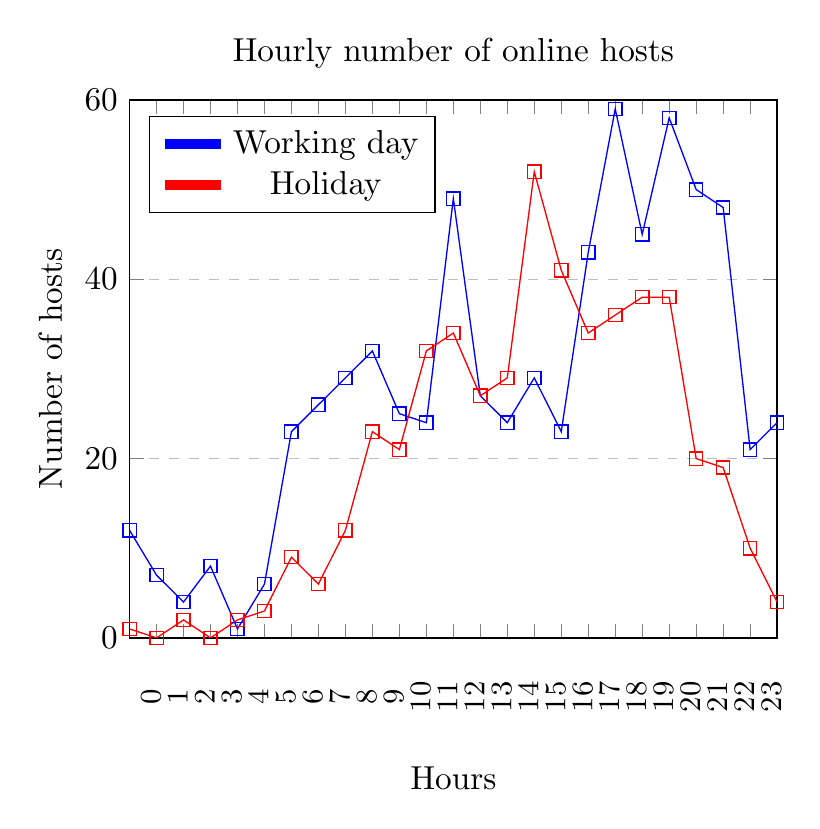
\begin{tikzpicture}[scale=1.2]
  \begin{axis}[
      title={Hourly number of online hosts},
      xlabel={Hours},
      ylabel={Number of hosts},
      xmin=0, xmax=24,
      ymin=0, ymax=60,
      x tick label style = {font = \small, text width = 1cm, align = center, rotate = 90, anchor = north east},
      xtick={0,1,2,3,4,5, 6, 7, 8, 9, 10, 11, 12, 13, 14, 15, 16, 17, 18, 19, 20, 21, 22, 23},
      ytick={0,20,40,60,80,100,120},
      legend pos=north west,
      ymajorgrids=true,
      grid style=dashed,
  ]
  \addlegendimage{draw=blue,mark=none, line width=3pt, color=blue},
  \addlegendentry{Working day},
  \addlegendimage{line width=3pt, color=red},
  \addlegendentry{Holiday},
  \addplot[
      color=blue,
      mark=square,
      ]
      coordinates {
      (0,12)(1,7)(2,4)(3,8)(4,1)(5,6)(6,23)(7,26)(8,29)(9,32)(10,25)(11,24)(12,49)(13,27)(14,24)(15,29)(16,23)(17,43)(18,59)(19,45)(20,58)(21,50)(22,48)(23,21)(24,24)
      };
      \label{Working Day}
      
   \addplot[
      color=red,
      mark=square,
      ]
      coordinates {
      (0,1)(1,0)(2,2)(3,0)(4,2)(5,3)(6,9)(7,6)(8,12)(9,23)(10,21)(11,32)(12,34)(13,27)(14,29)(15,52)(16,41)(17,34)(18,36)(19,38)(20,38)(21,20)(22,19)(23,10)(24,4)
      };
      \label{Holiday}
  \end{axis}
  \end{tikzpicture}
\end{center}

We can see through the graph that the number of online hosts is low after midnight and suddenly rises at 6 AM. The number of online hosts then again decreases and rises at 12 noon (lunch break). There is again a low till 5 PM in the afternoon and remains high thereon till 10 PM after which it starts falling again. For holidays the trend is more evenly spread.

To find the servers running on the same LAN the command \textit{nmap –n 10.208.26.0/24} was used. The result of this command can be found in the appendix \ref{appendix:nmap_local_servers}. A trimmed version for one server is shown below:

\begin{lstlisting}[style=BashInputStyle]
C:\Users\Shreshth Tuli\source>nmap -n 10.208.26.0/24
Nmap scan report for 10.208.26.1
Host is up (0.0073s latency).
Not shown: 997 closed ports
PORT   STATE SERVICE
22/tcp open  ssh
23/tcp open  telnet
80/tcp open  http
\end{lstlisting}

To find the OS running on the systems the command the command \textit{nmap –n –O 10.208.26.145}. Like for the IP 10.208.26.145 the result is:

\begin{lstlisting}[style=BashInputStyle]
Nmap scan report for 10.208.26.145
Host is up (0.018s latency).
Not shown: 998 closed ports
PORT     STATE SERVICE
22/tcp   open  ssh
3389/tcp open  ms-wbt-server
No exact OS matches for host (If you know what OS is running on it, see https://nmap.org/submit/ ).
TCP/IP fingerprint:
OS:SCAN(V=7.70%E=4%D=8/14%OT=22%CT=1%CU=35522%PV=Y%DS=4%DC=I%G=Y%TM=5B72825
OS:0%P=i686-pc-windows-windows)SEQ(SP=FC%GCD=1%ISR=10D%TI=Z%CI=I%II=I%TS=A)
OS:SEQ(CI=I%II=I)OPS(O1=M218ST11NW7%O2=M218ST11NW7%O3=M218NNT11NW7%O4=M218S
OS:T11NW7%O5=M218ST11NW7%O6=M218ST11)WIN(W1=7120%W2=7120%W3=7120%W4=7120%W5
OS:=7120%W6=7120)ECN(R=Y%DF=Y%T=40%W=7210%O=M218NNSNW7%CC=Y%Q=)T1(R=Y%DF=Y%
OS:T=40%S=O%A=S+%F=AS%RD=0%Q=)T2(R=N)T3(R=N)T4(R=Y%DF=Y%T=40%W=0%S=A%A=Z%F=
OS:R%O=%RD=0%Q=)T5(R=Y%DF=Y%T=40%W=0%S=Z%A=S+%F=AR%O=%RD=0%Q=)T6(R=Y%DF=Y%T
OS:=40%W=0%S=A%A=Z%F=R%O=%RD=0%Q=)T7(R=Y%DF=Y%T=40%W=0%S=Z%A=S+%F=AR%O=%RD=
OS:0%Q=)U1(R=Y%DF=N%T=40%IPL=164%UN=0%RIPL=G%RID=G%RIPCK=G%RUCK=G%RUD=G)IE(
OS:R=Y%DFI=N%T=40%CD=S)

Network Distance: 4 hops
\end{lstlisting}

This was a Windows based system and different details have been returned by the nmap command.

\newpage

\section{Part B - Network Topologies}

Mininet is a network emulator that runs a collection of end-hosts, switches, router, and links on
the single Linux kernel and gives virtualization of a network on a single system. Different topologies including linear, ring, mesh and star were built using the Python API of Mininet. The source code for developing the files can be read at appendix \ref{appendix:python}. Different tests were performed on these topologies with Mininet CLI commands given in appendix \ref{appendix:mininet_commands}. These tests were also performed in different scenarios when distinct parameter values of bandwidth, delay, packet loss percentage, maximum queue length. 

\subsection{Linear Topology}

The Linear topology is the simplest topology where all hosts are connected linearly like a bus as shown in the figure below.

\begin{figure}[h]
\centering % Center table
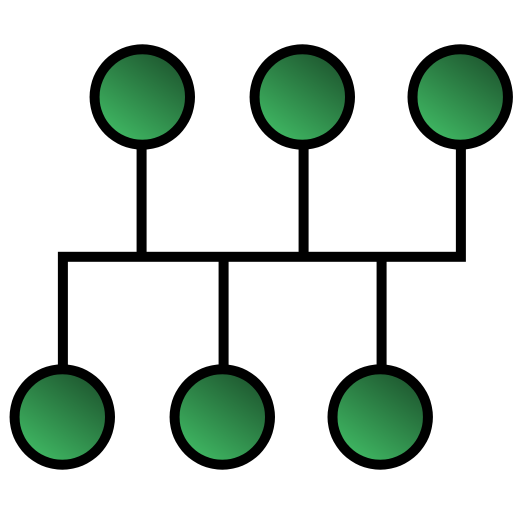
\includegraphics[width=5cm]{linear}
\end{figure}

The test results on this topology can be seen in appendix \ref{appendix:linear}. The ping connectivity showed no problem in reachability of the nodes. The network latency was low - around 0.5ms for each ping. The bandwidth for default case was nearly 17 Gbit/sec. the switches could \textit{nslookup} Google server but hosts couldn't. The latency for far away hosts (h1 and h10) is more than those adjacent to each other (h1 and h2).

For different scenarios:
\begin{enumerate}
\item Bandwidth limited to 10 Mb/s : The \textit{iperf} command showed significant reduction of bandwidth from 10 Gb/s to 10 Mb/s. Bandwidths of distant and close hosts (in terms of number of switches in between) remained same before after after limiting the bandwidth.
\item Delay limited to 5 ms : Clearly the latency of ping has significantly increased from nearly 0.5 ms to 5.30 ms for adjacent hosts and 8.7 ms for far off hosts (h1 and h10). The effective bandwidth remains nearly same.
\item Loss percentage 2\% : The ping reachability for this case is not 100\% as expected. The \textit{pingall} command outputs 22\% packets dropped. Even the ping RTT increases from 0.5 ms (in default case) to 2 ms for adjacent hosts and upto 10 ms for far away hosts (h1 and h10). The bandwidth is also lower - around 55 Mb/s compared to 18 Gb/s in default case. All this is due to packet drops and thus retransmission which leads to reduction in performance.
\item Max queue length limited to 2 packets : Does not lead to much change due to low network traffic. For high network traffic situations like in mesh network some packets are dropped so leads to downgrade of network performance but not in this case. The latency and effective bandwidths remain nearly same.
\end{enumerate}


\subsection{Ring Topology}

The Ring topology is a simple topology where all hosts are connected in a ring fashion as shown in the figure below.

\begin{figure}[h]
\centering % Center table

\includegraphics[width=5cm]{ring}
\end{figure}

The test results on this topology can be seen in appendix \ref{appendix:ring}. The ping connectivity showed no problem in reachability of the nodes. The network latency was low - around 0.5ms for each ping. The bandwidth for default case was nearly 17 Gbit/sec. the switches could \textit{nslookup} Google server but hosts couldn't. Unlike the linear topology, the latency differs in different sense. For hosts along the diameter (h1 and h5) the latency is maximum and how adjacent (h1 and h2, h1 and h10) minimum.

For different scenarios:
\begin{enumerate}
\item Bandwidth limited to 10 Mb/s : The \textit{iperf} command showed significant reduction of bandwidth from 17 Gb/s to 10 Mb/s. Bandwidths of distant and close hosts (in terms of number of switches in between) remained almost same before after after limiting the bandwidth.
\item Delay limited to 5 ms : Clearly the latency of ping has significantly increased from nearly 0.5 ms to 5.30 ms for adjacent hosts and 7.95 ms for far off hosts (h1 and h5). The increase is lower than in linear topology as the maximum number of intermediary nodes in linear is 8 but in ring is 3. The effective bandwidth remains nearly same.
\item Loss percentage 2\% : The ping reachability for this case is not 100\% as expected. The \textit{pingall} command outputs 22\% packets dropped which is same as the linear case. Even the ping RTT increases from 0.5 ms (in default case) to 3.3 ms for adjacent hosts and upto 5.1 ms for far away hosts (h1 and h5). The bandwidth is also lower - around 41 Mb/s for adjacent and 5 Mb/s for far away, compared to 18 Gb/s in default case. All this is due to packet drops and thus retransmission which leads to reduction in performance.
\item Max queue length limited to 2 packets : Does not lead to much change due to low network traffic.
\end{enumerate}

\newpage

\subsection{Mesh Topology}

The Mesh topology is a topology where all every host is connected to every other host (in fully meshed toplogy) as shown in the figure below.

\begin{figure}[h]
\centering % Center table
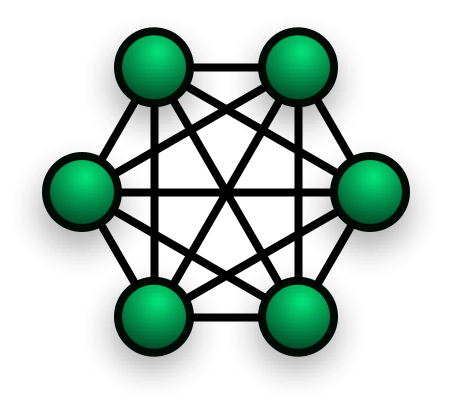
\includegraphics[width=5cm]{mesh}
\end{figure}

The test results on this topology can be seen in appendix \ref{appendix:mesh}. The ping connectivity showed no problem in reachability of the nodes. The network latency was low - around 0.2ms for each ping. The bandwidth for default case was nearly 19 Gbit/sec. the switches could \textit{nslookup} Google server but hosts couldn't. Unlike the linear or ring topologies, the latency does not change in a full-mesh topology as each host is adjacent to every other host. Due to Minimum spanning tree path in the controller, there is inherent difference in latencies due to difference in the depths (of tree) of the nodes.

For different scenarios:
\begin{enumerate}
\item Bandwidth limited to 10 Mb/s : The \textit{iperf} command showed significant reduction of bandwidth from 19 Gb/s to 10 Mb/s. Bandwidths between any two pairs of hosts is same.
\item Delay limited to 5 ms : Clearly the latency of ping has significantly increased from nearly 0.2 ms to 17  ms which is same for every pair as each pair is adjacent.
\item Loss percentage 2\% : The ping reachability for this case is not 100\% as expected. The \textit{pingall} command outputs 14\% packets dropped which is left than the linear/ring case due to multiple paths now available. Even the ping RTT increases from 0.1 ms to nearly 3 ms (for all pairs). The bandwidth is also lower - around 40 Mb/s, compared to 19 Gb/s in default case. All this is due to packet drops and thus retransmission which leads to reduction in performance.
\item Max queue length limited to 2 packets : Leads to packet drops in the network as shown by \textit{pingall} command. The packet drop may be due to congestion in the network as many nodes are connected and different routes are used for sending packets. If many nodes send simultaneously there is high chances of congestion due to only 2 packet queue length limit.
\end{enumerate}

\newpage

\subsection{Star Topology}

The Star topology is a simple topology where all hosts are connected to a single switch as shown in the figure below.

\begin{figure}[h]
\centering % Center table

\includegraphics[width=5cm]{star}
\end{figure}

The test results on this topology can be seen in appendix \ref{appendix:star}. The ping connectivity showed no problem in reachability of the nodes. The network latency was low - around 0.1ms for each ping. This is lowest among all nodes due to only one switch in between each node and low network load. The bandwidth for default case was nearly 19 Gbit/sec. The switches could \textit{nslookup} Google server but hosts couldn't. Latency for all pairs is same unlike linear/ring topologies. There is no biasing based on the number of switches in between as each host is connected to the same switch, so changes in values are uniform across all hosts.

For different scenarios:
\begin{enumerate}
\item Bandwidth limited to 10 Mb/s : The \textit{iperf} command showed significant reduction of bandwidth from 19 Gb/s to 9.9 Mb/s. Bandwidths between different pairs remains same.
\item Delay limited to 5 ms : Clearly the latency of ping has significantly increased from nearly 0.1 ms to 4.4 ms for each pair. The increase is lower than in linear topology as the maximum number of intermediary nodes in linear is 8 but in here it is only 1. The effective bandwidth remains nearly same.
\item Loss percentage 2\% : The ping reachability for this case is not 100\% as expected. The \textit{pingall} command outputs 7\% packets dropped which is much lower than the previous cases which is due to only 1 switch in between so cumulative packet loss is less. Other topologies have multiple links in between hosts and each link has loss percentage which cumulates along the network path. Even the ping RTT increases from 0.1 ms (in default case) to 1 ms for each pair of hosts. The bandwidth is also lower - around 192 Mb/s, compared to 19 Gb/s in default case. Drop in bandwidth is lower also due to the previous argument. All this is due to packet drops and thus retransmission which leads to reduction in performance but lower due to lesser links.
\item Max queue length limited to 2 packets : Does not lead to much change due to low network traffic and all hosts being adjacent to each other.
\end{enumerate}


\newpage

\subsection{Tabular Comparison}

Latency comparison of different scenarios:\\ \\

\begin{tabular}{|c|c|c|c|c|c|c|}
\hline 
\multicolumn{7}{|c|}{LATENCY (ms)}\tabularnewline
\hline 
\hline 
 & Default & BW = 10 Mb/s & Delay = 5ms & Loss = 2\% & Queue = 2 & Deviation\tabularnewline
\hline 
Linear & 0.5 & 0.5 & 7 & 7.2 & 0.5 & Yes\tabularnewline
\hline 
Ring & 0.6 & 0.6 & 5.3 & 4 & 0.5 & Yes\tabularnewline
\hline 
Mesh & 0.2 & 0.2 & 17 & 3 & 5 & No\tabularnewline
\hline 
Star & 0.1 & 0.1 & 4.7 & 1 & 0.1 & No\tabularnewline
\hline 
\end{tabular}\\ \\

\noindent
Bandwidth comparison of different scenarios:\\ \\

\begin{tabular}{|c|c|c|c|c|c|c|}
\hline 
\multicolumn{7}{|c|}{BANDWIDTH }\tabularnewline
\hline 
\hline 
 & Default & BW = 10 Mb/s & Delay = 5ms & Loss = 2\% & Queue = 2 & Deviation\tabularnewline
\hline 
Linear & 17 Gb/s & 10 Mb/s & 13 Gb/s & 55 Mb/s & 17 Gb/s & No\tabularnewline
\hline 
Ring & 17 Gb/s & 10 Mb/s & 7 Gb/s & 41 Mb/s & 17 Gb/s & Yes\tabularnewline
\hline 
Mesh & 19 Gb/s  & 10 Mb/s & 12 Gb/s & 40 Mb/s  & 18 Gb/s & No\tabularnewline
\hline 
Star & 19 Gb/s  & 10 Mb/s & 14.7 Gb/s & 192 Mb/s & 19 Gb/s & No\tabularnewline
\hline 
\end{tabular}



\newpage

\begin{appendices}

\section{Part A}

\subsection{Experiments with ping}
\label{appendix:ping}
\begin{lstlisting}[style=BashInputStyle]
C:\Users\Shreshth Tuli\source>ping www.google.com

Pinging www.google.com [216.58.221.36] with 32 bytes of data:
Reply from 216.58.221.36: bytes=32 time=5ms TTL=50
Reply from 216.58.221.36: bytes=32 time=5ms TTL=50
Reply from 216.58.221.36: bytes=32 time=5ms TTL=50
Reply from 216.58.221.36: bytes=32 time=6ms TTL=50

Ping statistics for 216.58.221.36:
    Packets: Sent = 4, Received = 4, Lost = 0 (0% loss),
Approximate round trip times in milli-seconds:
    Minimum = 5ms, Maximum = 6ms, Average = 5ms
\end{lstlisting}  

\begin{lstlisting}[style=BashInputStyle]
C:\Users\Shreshth Tuli\source>ping www.harvard.edu

Pinging www.harvard.edu.cdn.cloudflare.net [104.16.155.6] with 32 bytes of data:
Reply from 104.16.155.6: bytes=32 time=46ms TTL=52
Reply from 104.16.155.6: bytes=32 time=47ms TTL=52
Reply from 104.16.155.6: bytes=32 time=46ms TTL=52
Reply from 104.16.155.6: bytes=32 time=46ms TTL=52

Ping statistics for 104.16.155.6:
    Packets: Sent = 4, Received = 4, Lost = 0 (0% loss),
Approximate round trip times in milli-seconds:
    Minimum = 46ms, Maximum = 47ms, Average = 46ms
\end{lstlisting}  

\begin{lstlisting}[style=BashInputStyle]
C:\Users\Shreshth Tuli\source>ping www.iitd.ac.in

Pinging www.iitd.ac.in [10.7.174.111] with 32 bytes of data:
Reply from 10.7.174.111: bytes=32 time=2ms TTL=61
Reply from 10.7.174.111: bytes=32 time=3ms TTL=61
Reply from 10.7.174.111: bytes=32 time=2ms TTL=61
Reply from 10.7.174.111: bytes=32 time=2ms TTL=61

Ping statistics for 10.7.174.111:
    Packets: Sent = 4, Received = 4, Lost = 0 (0% loss),
Approximate round trip times in milli-seconds:
    Minimum = 2ms, Maximum = 3ms, Average = 2ms
\end{lstlisting}

\subsection{ifconfig network command}
\label{appendix:ifconfig}

\begin{lstlisting}[style=BashInputStyle]
C:\Users\Shreshth Tuli\source>ipconfig /all

Windows IP Configuration

   Host Name . . . . . . . . . . . . : DESKTOP-0I0PA3Q
   Primary Dns Suffix  . . . . . . . :
   Node Type . . . . . . . . . . . . : Hybrid
   IP Routing Enabled. . . . . . . . : No
   WINS Proxy Enabled. . . . . . . . : No

Wireless LAN adapter Local Area Connection* 1:

   Media State . . . . . . . . . . . : Media disconnected
   Connection-specific DNS Suffix  . :
   Description . . . . . . . . . . . : Microsoft Wi-Fi Direct Virtual Adapter
   Physical Address. . . . . . . . . : 9E-B6-D0-E4-4B-5F
   DHCP Enabled. . . . . . . . . . . : Yes
   Autoconfiguration Enabled . . . . : Yes

Wireless LAN adapter Local Area Connection* 2:

   Media State . . . . . . . . . . . : Media disconnected
   Connection-specific DNS Suffix  . :
   Description . . . . . . . . . . . : Microsoft Wi-Fi Direct Virtual Adapter #2
   Physical Address. . . . . . . . . : AE-B6-D0-E4-4B-5F
   DHCP Enabled. . . . . . . . . . . : Yes
   Autoconfiguration Enabled . . . . : Yes

Wireless LAN adapter Wi-Fi:

   Connection-specific DNS Suffix  . :
   Description . . . . . . . . . . . : Killer Wireless-n/a/ac 1535 Wireless Network Adapter
   Physical Address. . . . . . . . . : 9C-B6-D0-E4-4B-5F
   DHCP Enabled. . . . . . . . . . . : Yes
   Autoconfiguration Enabled . . . . : Yes
   Link-local IPv6 Address . . . . . : fe80::9c2f:be9d:dbb8:e3a2%9(Preferred)
   IPv4 Address. . . . . . . . . . . : 192.168.1.10(Preferred)
   Subnet Mask . . . . . . . . . . . : 255.255.255.0
   Lease Obtained. . . . . . . . . . : Friday, August 17, 2018 1:54:20 PM
   Lease Expires . . . . . . . . . . : Monday, August 20, 2018 4:18:33 PM
   Default Gateway . . . . . . . . . : fe80::76da:daff:fed2:92e6%9
                                       192.168.1.1
   DHCP Server . . . . . . . . . . . : 192.168.1.1
   DHCPv6 IAID . . . . . . . . . . . : 43824848
   DHCPv6 Client DUID. . . . . . . . : 00-01-00-01-21-CB-0D-F2-9C-B6-D0-E4-4B-5F
   DNS Servers . . . . . . . . . . . : 202.56.215.54
                                       59.144.144.100
   NetBIOS over Tcpip. . . . . . . . : Enabled
\end{lstlisting}

\subsection{NMAP - number of online hosts}
\label{appendix:nmap_online}
\begin{lstlisting}[style=BashInputStyle]
C:\Users\Shreshth Tuli\source>nmap -n -sP 10.194.6.0/24
Starting Nmap 7.70 ( https://nmap.org ) at 2018-08-14 12:43 India Standard Time
Nmap scan report for 10.194.6.13
Host is up (0.024s latency).
MAC Address: 4C:49:E3:72:B5:95 (Xiaomi Communications)
Nmap scan report for 10.194.6.19
Host is up (0.0050s latency).
MAC Address: AC:29:3A:E7:89:A4 (Apple)
Nmap scan report for 10.194.6.21
Host is up (0.0010s latency).
MAC Address: 74:23:44:41:06:0F (Xiaomi Communications)
Nmap scan report for 10.194.6.43
Host is up (0.0060s latency).
MAC Address: 64:A2:F9:0B:14:B2 (Unknown)
Nmap scan report for 10.194.6.56
Host is up (0.013s latency).
MAC Address: F8:2F:A8:DD:C9:55 (Hon Hai Precision Ind.)
Nmap scan report for 10.194.6.63
Host is up (0.028s latency).
MAC Address: B4:EF:FA:14:2F:E1 (Lemobile Information Technology (Beijing))
Nmap scan report for 10.194.6.67
Host is up (0.023s latency).
MAC Address: DC:72:9B:6F:D3:CA (Unknown)
Nmap scan report for 10.194.6.73
Host is up (0.0060s latency).
MAC Address: EC:D0:9F:56:09:49 (Xiaomi Communications)
Nmap scan report for 10.194.6.75
Host is up (0.039s latency).
MAC Address: 20:82:C0:F5:F7:45 (Xiaomi Communications)
Nmap scan report for 10.194.6.91
Host is up (0.032s latency).
MAC Address: D8:32:E3:63:81:5A (Unknown)
Nmap scan report for 10.194.6.109
Host is up (0.0090s latency).
MAC Address: 38:E6:0A:1A:22:91 (Unknown)
Nmap scan report for 10.194.6.132
Host is up (0.016s latency).
MAC Address: C8:25:E1:22:81:A6 (Lemobile Information Technology (Beijing))
Nmap scan report for 10.194.6.134
Host is up (0.010s latency).
MAC Address: EC:D0:9F:3B:90:82 (Xiaomi Communications)
Nmap scan report for 10.194.6.143
Host is up (0.022s latency).
MAC Address: 38:E6:0A:D9:EA:22 (Unknown)
Nmap scan report for 10.194.6.145
Host is up (0.018s latency).
MAC Address: 50:8F:4C:9A:0E:97 (Xiaomi Communications)
Nmap scan report for 10.194.6.151
Host is up (0.0050s latency).
MAC Address: 6C:AB:31:4C:99:F4 (Apple)
Nmap scan report for 10.194.6.152
Host is up (0.0010s latency).
MAC Address: A8:96:75:5B:85:80 (Motorola Mobility, a Lenovo Company)
Nmap scan report for 10.194.6.158
Host is up (0.013s latency).
MAC Address: CC:2D:B7:F1:5F:F3 (Unknown)
Nmap scan report for 10.194.6.163
Host is up (0.010s latency).
MAC Address: 64:A2:F9:58:D5:E9 (Unknown)
Nmap scan report for 10.194.6.176
Host is up (0.020s latency).
MAC Address: 10:08:B1:D2:50:C3 (Hon Hai Precision Ind.)
Nmap scan report for 10.194.6.193
Host is up (0.021s latency).
MAC Address: D8:9A:34:76:B4:B8 (Beijing Shenqi Technology)
Nmap scan report for 10.194.6.201
Host is up (0.0040s latency).
MAC Address: EC:51:BC:4C:4D:1B (Guangdong Oppo Mobile Telecommunications)
Nmap scan report for 10.194.6.212
Host is up (0.024s latency).
MAC Address: C0:EE:FB:73:2B:EF (OnePlus Tech (Shenzhen))
Nmap scan report for 10.194.6.221
Host is up (0.0060s latency).
MAC Address: D8:32:E3:60:0E:0E (Unknown)
Nmap scan report for 10.194.6.229
Host is up (0.012s latency).
MAC Address: D0:04:01:21:A9:13 (Motorola Mobility, a Lenovo Company)
Nmap scan report for 10.194.6.236
Host is up (0.0070s latency).
MAC Address: 60:6C:66:AF:BC:75 (Intel Corporate)
Nmap scan report for 10.194.6.238
Host is up (0.0030s latency).
MAC Address: 40:4E:36:87:9E:FD (HTC)
Nmap scan report for 10.194.6.241
Host is up (0.021s latency).
MAC Address: 6C:AB:31:4B:F3:D4 (Apple)
Nmap scan report for 10.194.6.245
Host is up (0.015s latency).
MAC Address: A0:56:F3:F1:32:8F (Unknown)
Nmap scan report for 10.194.6.251
Host is up.
Nmap done: 256 IP addresses (30 hosts up) scanned in 2.26 seconds
\end{lstlisting}  


\subsection{NMAP servers on same LAN}
\label{appendix:nmap_local_servers}

\begin{lstlisting}[style=BashInputStyle]
C:\Users\Shreshth Tuli\source>nmap -n 10.208.26.0/24
Nmap scan report for 10.208.26.1
Host is up (0.0073s latency).
Not shown: 997 closed ports
PORT   STATE SERVICE
22/tcp open  ssh
23/tcp open  telnet
80/tcp open  http

Nmap scan report for 10.208.26.145
Host is up (0.0073s latency).
Not shown: 998 closed ports
PORT     STATE SERVICE
22/tcp   open  ssh
3389/tcp open  ms-wbt-server

Nmap scan report for 10.208.26.146
Host is up (0.012s latency).
All 1000 scanned ports on 10.208.26.146 are filtered

Nmap scan report for 10.208.26.148
Host is up (0.0074s latency).
Not shown: 999 closed ports
PORT     STATE SERVICE
5900/tcp open  vnc

Nmap scan report for 10.208.26.160
Host is up (0.0091s latency).
All 1000 scanned ports on 10.208.26.160 are closed

Nmap scan report for 10.208.26.165
Host is up (0.0093s latency).
Not shown: 998 closed ports
PORT     STATE SERVICE
22/tcp   open  ssh
3389/tcp open  ms-wbt-server

Nmap scan report for 10.208.26.169
Host is up (0.023s latency).
All 1000 scanned ports on 10.208.26.169 are closed (633) or filtered (367)

Nmap scan report for 10.208.26.170
Host is up (0.017s latency).
Not shown: 991 filtered ports
PORT      STATE  SERVICE
135/tcp   open   msrpc
3389/tcp  open   ms-wbt-server
49152/tcp open   unknown
49153/tcp open   unknown
49154/tcp open   unknown
49155/tcp open   unknown
49156/tcp open   unknown
49157/tcp open   unknown
49158/tcp closed unknown

Nmap scan report for 10.208.26.175
Host is up (0.0056s latency).
Not shown: 995 closed ports
PORT     STATE SERVICE
80/tcp   open  http
443/tcp  open  https
515/tcp  open  printer
631/tcp  open  ipp
9100/tcp open  jetdirect

Nmap scan report for 10.208.26.179
Host is up (0.0094s latency).
Not shown: 995 closed ports
PORT     STATE SERVICE
80/tcp   open  http
554/tcp  open  rtsp
880/tcp  open  unknown
8000/tcp open  http-alt
9010/tcp open  sdr

Nmap scan report for 10.208.26.184
Host is up (0.0064s latency).
Not shown: 999 closed ports
PORT   STATE SERVICE
22/tcp open  ssh

Nmap scan report for 10.208.26.187
Host is up (0.0064s latency).
Not shown: 999 closed ports
PORT   STATE SERVICE
22/tcp open  ssh

Nmap scan report for 10.208.26.201
Host is up (0.0082s latency).
Not shown: 998 closed ports
PORT     STATE SERVICE
80/tcp   open  http
5900/tcp open  vnc

Nmap scan report for 10.208.26.202
Host is up (0.0020s latency).
All 1000 scanned ports on 10.208.26.202 are closed

Nmap scan report for 10.208.26.211
Host is up (0.0078s latency).
All 1000 scanned ports on 10.208.26.211 are closed

Nmap scan report for 10.208.26.216
Host is up (0.0021s latency).
Not shown: 997 filtered ports
PORT     STATE SERVICE
25/tcp   open  smtp
515/tcp  open  printer
9100/tcp open  jetdirect

Nmap scan report for 10.208.26.221
Host is up (0.0054s latency).
All 1000 scanned ports on 10.208.26.221 are closed

Nmap scan report for 10.208.26.222
Host is up (0.0071s latency).
Not shown: 995 closed ports
PORT     STATE SERVICE
80/tcp   open  http
554/tcp  open  rtsp
880/tcp  open  unknown
8000/tcp open  http-alt
9010/tcp open  sdr

Nmap scan report for 10.208.26.224
Host is up (0.026s latency).
All 1000 scanned ports on 10.208.26.224 are filtered

Nmap scan report for 10.208.26.238
Host is up (0.010s latency).
All 1000 scanned ports on 10.208.26.238 are closed

Nmap scan report for 10.208.26.241
Host is up (0.0079s latency).
Not shown: 998 closed ports
PORT     STATE SERVICE
22/tcp   open  ssh
3389/tcp open  ms-wbt-server

Nmap scan report for 10.208.26.248
Host is up (0.0090s latency).
Not shown: 999 closed ports
PORT     STATE SERVICE
3389/tcp open  ms-wbt-server

Nmap scan report for 10.208.26.254
Host is up (0.0097s latency).
Not shown: 993 closed ports
PORT      STATE SERVICE
135/tcp   open  msrpc
139/tcp   open  netbios-ssn
445/tcp   open  microsoft-ds
49152/tcp open  unknown
49153/tcp open  unknown
49154/tcp open  unknown
49160/tcp open  unknown

Nmap done: 256 IP addresses (23 hosts up) scanned in 606.66 seconds
\end{lstlisting}

\section{Part B}
\subsection{Python Code}
\label{appendix:python}
\begin{lstlisting}[language=python]
"""
Mininet Topologies with 10 nodes 
Author : Shreshth Tuli

Usage:

1. Linear Topology
    - sudo mn --custom topos.py --topo linear
2. Ring Topology
    - sudo mn --custom topos.py --topo ring --controller=remote,ip=127.0.0.1
3. Mesh Topology
    - sudo mn --custom topos.py --topo mesh --controller=remote,ip=127.0.0.1
4. Star Topology
    - sudo mn --custom topos.py --topo star
"""

from mininet.topo import Topo

class LinearTopo( Topo ):
    "Linear Topology Mininet"

    def __init__( self ):

        # Initialize topology
        Topo.__init__( self )

        hosts = []
        switches = []

        for x in range(0, 10):

            # Add hosts and switches
            hosts.append(self.addHost( 'h%s' % (x+1) ))
            switches.append(self.addSwitch( 's%s' % (x+1) ))

            # Add links in linear topology

            # Connecting hosts to switches
            self.addLink(hosts[x], switches[x])
            # Connecting switches in linear order
            if(x > 0):
                self.addLink(switches[x-1], switches[x])

class LinearTopo2( Topo ):
    "Linear Topology Mininet with different parameters"

    def __init__( self ):

        # Initialize topology
        Topo.__init__( self )

        self.hosts = []
        self.switches = []

        for x in range(0, 10):

            # Add hosts and switches
            self.hosts.append(self.addHost( 'h%s' % (x+1) ))
            self.switches.append(self.addSwitch( 's%s' % (x+1) ))

            # Connecting hosts to switches
            self.addLink(self.hosts[x], self.switches[x])
        
        for x in range(5, 9):
            self.addLink(self.switches[x], self.switches[x+1])

        self.build()

    def build(self):
        # Adding links between switches with different paraneters
        self.addLink(self.switches[0], self.switches[1])
        self.addLink(self.switches[1], self.switches[2], bw=10)
        self.addLink(self.switches[2], self.switches[3], delay='5ms')
        self.addLink(self.switches[3], self.switches[4], loss=2)
        self.addLink(self.switches[4], self.switches[5], max_queue_size=2)


class RingTopo( Topo ):
    "Ring Topology Mininet"

    def __init__( self ):

        # Initialize topology
        Topo.__init__( self )

        hosts = []
        switches = []

        for x in range(0, 10):

            # Add hosts and switches
            hosts.append(self.addHost( 'h%s' % (x+1) ))
            switches.append(self.addSwitch( 's%s' % (x+1) ))

            # Add links in linear topology

            # Connecting hosts to switches
            self.addLink(hosts[x], switches[x])
            # Connecting switches in ring order
            if(x > 0):
                self.addLink(switches[x-1], switches[x])

        self.addLink(switches[0], switches[9])


class MeshTopo( Topo ):
    "Mesh Topology Mininet"

    def __init__( self ):

        # Initialize topology
        Topo.__init__( self )

        hosts = []
        switches = []

        for x in range(0, 10):

            # Add hosts and switches
            hosts.append(self.addHost( 'h%s' % (x+1) ))
            switches.append(self.addSwitch( 's%s' % (x+1) ))

            # Add links in mesh topology

            # Connecting hosts to switches
            self.addLink(hosts[x], switches[x])
            # Connecting switches in mesh order

        for x in range(0, 10):
            # Connecting switches in mesh order
            for y in range(x+1, 10):
                self.addLink(switches[x], switches[y])


class StarTopo( Topo ):
    "Star Topology Mininet"

    def __init__( self ):

        # Initialize topology
        Topo.__init__( self )

        hosts = []
        # Add common switch
        switch = self.addSwitch( 's1' )

        for x in range(0, 10):
            # Add hosts
            hosts.append(self.addHost( 'h%s' % (x+1) ))
            # Connect host and switch
            self.addLink(hosts[x], switch)
   

topos = { 
 'linear': ( lambda: LinearTopo() ),
 'ring': ( lambda: RingTopo() ) ,
 'mesh': ( lambda: MeshTopo() ) ,
 'star': ( lambda: StarTopo())  }
\end{lstlisting}

\subsection{Mininet Commands}
\label{appendix:mininet_commands}

\begin{lstlisting}[style=BashInputStyle]
net
pingall
h1 ping -c 2 h2
h1 ping -c 2 h5
h1 ping -c 2 h10
iperf h1 h2
iperf h1 h5
iperf h1 h10
h1 ifconfig
h5 ifconfig
h10 ifconfig
h1 route
h5 route
h10 route
h1 traceroute h2
h1 traceroute h5
h1 traceroute h10
s1 nslookup www.google.com
\end{lstlisting}

\subsection{Linear Topology}
\label{appendix:linear}
\begin{lstlisting}[style=BashInputStyle]
mininet@mininet-vm:~/mininet/custom$ sudo mn --custom topos.py --topo linear
*** Creating network
*** Adding controller
*** Adding hosts:
h1 h2 h3 h4 h5 h6 h7 h8 h9 h10
*** Adding switches:
s1 s2 s3 s4 s5 s6 s7 s8 s9 s10
*** Adding links:
(h1, s1) (h2, s2) (h3, s3) (h4, s4) (h5, s5) (h6, s6) (h7, s7) (h8, s8) (h9, s9) (h10, s10) (s1, s2) (s2, s3) (s3, s4) (s4, s5) (s5, s6) (s6, s7) (s7, s8) (s8, s9) (s9, s10)
*** Configuring hosts
h1 h2 h3 h4 h5 h6 h7 h8 h9 h10
*** Starting controller
c0
*** Starting 10 switches
s1 s2 s3 s4 s5 s6 s7 s8 s9 s10 ...
*** Starting CLI:
mininet> net
h1 h1-eth0:s1-eth1
h2 h2-eth0:s2-eth1
h3 h3-eth0:s3-eth1
h4 h4-eth0:s4-eth1
h5 h5-eth0:s5-eth1
h6 h6-eth0:s6-eth1
h7 h7-eth0:s7-eth1
h8 h8-eth0:s8-eth1
h9 h9-eth0:s9-eth1
h10 h10-eth0:s10-eth1
s1 lo:  s1-eth1:h1-eth0 s1-eth2:s2-eth2
s2 lo:  s2-eth1:h2-eth0 s2-eth2:s1-eth2 s2-eth3:s3-eth2
s3 lo:  s3-eth1:h3-eth0 s3-eth2:s2-eth3 s3-eth3:s4-eth2
s4 lo:  s4-eth1:h4-eth0 s4-eth2:s3-eth3 s4-eth3:s5-eth2
s5 lo:  s5-eth1:h5-eth0 s5-eth2:s4-eth3 s5-eth3:s6-eth2
s6 lo:  s6-eth1:h6-eth0 s6-eth2:s5-eth3 s6-eth3:s7-eth2
s7 lo:  s7-eth1:h7-eth0 s7-eth2:s6-eth3 s7-eth3:s8-eth2
s8 lo:  s8-eth1:h8-eth0 s8-eth2:s7-eth3 s8-eth3:s9-eth2
s9 lo:  s9-eth1:h9-eth0 s9-eth2:s8-eth3 s9-eth3:s10-eth2
s10 lo:  s10-eth1:h10-eth0 s10-eth2:s9-eth3
c0
mininet> pingall
*** Ping: testing ping reachability
h1 -> h2 h3 h4 h5 h6 h7 h8 h9 h10
h2 -> h1 h3 h4 h5 h6 h7 h8 h9 h10
h3 -> h1 h2 h4 h5 h6 h7 h8 h9 h10
h4 -> h1 h2 h3 h5 h6 h7 h8 h9 h10
h5 -> h1 h2 h3 h4 h6 h7 h8 h9 h10
h6 -> h1 h2 h3 h4 h5 h7 h8 h9 h10
h7 -> h1 h2 h3 h4 h5 h6 h8 h9 h10
h8 -> h1 h2 h3 h4 h5 h6 h7 h9 h10
h9 -> h1 h2 h3 h4 h5 h6 h7 h8 h10
h10 -> h1 h2 h3 h4 h5 h6 h7 h8 h9
*** Results: 0% dropped (90/90 received)
mininet> h1 ping -c 2 h2
PING 10.0.0.2 (10.0.0.2) 56(84) bytes of data.
64 bytes from 10.0.0.2: icmp_seq=1 ttl=64 time=0.546 ms
64 bytes from 10.0.0.2: icmp_seq=2 ttl=64 time=0.694 ms

--- 10.0.0.2 ping statistics ---
2 packets transmitted, 2 received, 0% packet loss, time 1001ms
rtt min/avg/max/mdev = 0.546/0.620/0.694/0.074 ms
mininet> h1 ping -c 2 h5
PING 10.0.0.5 (10.0.0.5) 56(84) bytes of data.
64 bytes from 10.0.0.5: icmp_seq=1 ttl=64 time=0.459 ms
64 bytes from 10.0.0.5: icmp_seq=2 ttl=64 time=0.106 ms

--- 10.0.0.5 ping statistics ---
2 packets transmitted, 2 received, 0% packet loss, time 1002ms
rtt min/avg/max/mdev = 0.106/0.282/0.459/0.177 ms
mininet> h1 ping -c 2 h10
PING 10.0.0.10 (10.0.0.10) 56(84) bytes of data.
64 bytes from 10.0.0.10: icmp_seq=1 ttl=64 time=0.480 ms
64 bytes from 10.0.0.10: icmp_seq=2 ttl=64 time=0.141 ms

--- 10.0.0.10 ping statistics ---
2 packets transmitted, 2 received, 0% packet loss, time 1002ms
rtt min/avg/max/mdev = 0.141/0.310/0.480/0.170 ms
mininet> iperf h1 h2
*** Iperf: testing TCP bandwidth between h1 and h2
.*** Results: ['17.8 Gbits/sec', '17.8 Gbits/sec']
mininet> iperf h1 h5
*** Iperf: testing TCP bandwidth between h1 and h5
*** Results: ['17.6 Gbits/sec', '17.6 Gbits/sec']
mininet> iperf h1 h10
*** Iperf: testing TCP bandwidth between h1 and h10
*** Results: ['15.9 Gbits/sec', '15.9 Gbits/sec']
mininet> h1 ifconfig
h1-eth0   Link encap:Ethernet  HWaddr 6e:3f:9c:41:46:85
          inet addr:10.0.0.1  Bcast:10.255.255.255  Mask:255.0.0.0
          UP BROADCAST RUNNING MULTICAST  MTU:1500  Metric:1
          RX packets:130231 errors:0 dropped:0 overruns:0 frame:0
          TX packets:562811 errors:0 dropped:0 overruns:0 carrier:0
          collisions:0 txqueuelen:1000
          RX bytes:8595642 (8.5 MB)  TX bytes:32085860502 (32.0 GB)

lo        Link encap:Local Loopback
          inet addr:127.0.0.1  Mask:255.0.0.0
          UP LOOPBACK RUNNING  MTU:65536  Metric:1
          RX packets:0 errors:0 dropped:0 overruns:0 frame:0
          TX packets:0 errors:0 dropped:0 overruns:0 carrier:0
          collisions:0 txqueuelen:0
          RX bytes:0 (0.0 B)  TX bytes:0 (0.0 B)

mininet> h5 ifconfig
h5-eth0   Link encap:Ethernet  HWaddr 0e:5c:af:e7:3c:b6
          inet addr:10.0.0.5  Bcast:10.255.255.255  Mask:255.0.0.0
          UP BROADCAST RUNNING MULTICAST  MTU:1500  Metric:1
          RX packets:193207 errors:0 dropped:0 overruns:0 frame:0
          TX packets:44949 errors:0 dropped:0 overruns:0 carrier:0
          collisions:0 txqueuelen:1000
          RX bytes:11014410438 (11.0 GB)  TX bytes:2966858 (2.9 MB)

lo        Link encap:Local Loopback
          inet addr:127.0.0.1  Mask:255.0.0.0
          UP LOOPBACK RUNNING  MTU:65536  Metric:1
          RX packets:0 errors:0 dropped:0 overruns:0 frame:0
          TX packets:0 errors:0 dropped:0 overruns:0 carrier:0
          collisions:0 txqueuelen:0
          RX bytes:0 (0.0 B)  TX bytes:0 (0.0 B)

mininet> h10 ifconfig
h10-eth0  Link encap:Ethernet  HWaddr 02:9c:8e:3a:76:d7
          inet addr:10.0.0.10  Bcast:10.255.255.255  Mask:255.0.0.0
          UP BROADCAST RUNNING MULTICAST  MTU:1500  Metric:1
          RX packets:174724 errors:0 dropped:0 overruns:0 frame:0
          TX packets:40489 errors:0 dropped:0 overruns:0 carrier:0
          collisions:0 txqueuelen:1000
          RX bytes:9929787056 (9.9 GB)  TX bytes:2673386 (2.6 MB)

lo        Link encap:Local Loopback
          inet addr:127.0.0.1  Mask:255.0.0.0
          UP LOOPBACK RUNNING  MTU:65536  Metric:1
          RX packets:0 errors:0 dropped:0 overruns:0 frame:0
          TX packets:0 errors:0 dropped:0 overruns:0 carrier:0
          collisions:0 txqueuelen:0
          RX bytes:0 (0.0 B)  TX bytes:0 (0.0 B)

mininet> h1 route
Kernel IP routing table
Destination     Gateway         Genmask         Flags Metric Ref    Use Iface
10.0.0.0        *               255.0.0.0       U     0      0        0 h1-eth0
mininet> h5 route
Kernel IP routing table
Destination     Gateway         Genmask         Flags Metric Ref    Use Iface
10.0.0.0        *               255.0.0.0       U     0      0        0 h5-eth0
mininet> h10 route
Kernel IP routing table
Destination     Gateway         Genmask         Flags Metric Ref    Use Iface
10.0.0.0        *               255.0.0.0       U     0      0        0 h10-eth0
mininet> h1 traceroute h2
traceroute to 10.0.0.2 (10.0.0.2), 30 hops max, 60 byte packets
 1  10.0.0.2 (10.0.0.2)  3.989 ms  17.512 ms *
mininet> h1 traceroute h5
traceroute to 10.0.0.5 (10.0.0.5), 30 hops max, 60 byte packets
 1  10.0.0.5 (10.0.0.5)  15.849 ms * *
mininet> h1 traceroute h10
traceroute to 10.0.0.10 (10.0.0.10), 30 hops max, 60 byte packets
 1  10.0.0.10 (10.0.0.10)  35.827 ms * *
mininet> s1 nslookup www.google.com
Server:         202.56.215.54
Address:        202.56.215.54#53

Non-authoritative answer:
Name:   www.google.com
Address: 172.217.163.196
\end{lstlisting}

\subsection{Ring Topology}
\label{appendix:ring}
\begin{lstlisting}[style=BashInputStyle]
mininet@mininet-vm:~/mininet/custom$ sudo mn --custom topos.py --topo ring --controller=remote,ip=127.0.0.1
*** Creating network
*** Adding controller
Unable to contact the remote controller at 127.0.0.1:6653
Connecting to remote controller at 127.0.0.1:6633
*** Adding hosts:
h1 h2 h3 h4 h5 h6 h7 h8 h9 h10
*** Adding switches:
s1 s2 s3 s4 s5 s6 s7 s8 s9 s10
*** Adding links:
(h1, s1) (h2, s2) (h3, s3) (h4, s4) (h5, s5) (h6, s6) (h7, s7) (h8, s8) (h9, s9) (h10, s10) (s1, s2) (s1, s10) (s2, s3) (s3, s4) (s4, s5) (s5, s6) (s6, s7) (s7, s8) (s8, s9) (s9, s10)
*** Configuring hosts
h1 h2 h3 h4 h5 h6 h7 h8 h9 h10
*** Starting controller
c0
*** Starting 10 switches
s1 s2 s3 s4 s5 s6 s7 s8 s9 s10 ...
*** Starting CLI:
mininet> net
h1 h1-eth0:s1-eth1
h2 h2-eth0:s2-eth1
h3 h3-eth0:s3-eth1
h4 h4-eth0:s4-eth1
h5 h5-eth0:s5-eth1
h6 h6-eth0:s6-eth1
h7 h7-eth0:s7-eth1
h8 h8-eth0:s8-eth1
h9 h9-eth0:s9-eth1
h10 h10-eth0:s10-eth1
s1 lo:  s1-eth1:h1-eth0 s1-eth2:s2-eth2 s1-eth3:s10-eth3
s2 lo:  s2-eth1:h2-eth0 s2-eth2:s1-eth2 s2-eth3:s3-eth2
s3 lo:  s3-eth1:h3-eth0 s3-eth2:s2-eth3 s3-eth3:s4-eth2
s4 lo:  s4-eth1:h4-eth0 s4-eth2:s3-eth3 s4-eth3:s5-eth2
s5 lo:  s5-eth1:h5-eth0 s5-eth2:s4-eth3 s5-eth3:s6-eth2
s6 lo:  s6-eth1:h6-eth0 s6-eth2:s5-eth3 s6-eth3:s7-eth2
s7 lo:  s7-eth1:h7-eth0 s7-eth2:s6-eth3 s7-eth3:s8-eth2
s8 lo:  s8-eth1:h8-eth0 s8-eth2:s7-eth3 s8-eth3:s9-eth2
s9 lo:  s9-eth1:h9-eth0 s9-eth2:s8-eth3 s9-eth3:s10-eth2
s10 lo:  s10-eth1:h10-eth0 s10-eth2:s9-eth3 s10-eth3:s1-eth3
c0
mininet> pingall
*** Ping: testing ping reachability
h1 -> h2 h3 h4 h5 h6 h7 h8 h9 h10
h2 -> h1 h3 h4 h5 h6 h7 h8 h9 h10
h3 -> h1 h2 h4 h5 h6 h7 h8 h9 h10
h4 -> h1 h2 h3 h5 h6 h7 h8 h9 h10
h5 -> h1 h2 h3 h4 h6 h7 h8 h9 h10
h6 -> h1 h2 h3 h4 h5 h7 h8 h9 h10
h7 -> h1 h2 h3 h4 h5 h6 h8 h9 h10
h8 -> h1 h2 h3 h4 h5 h6 h7 h9 h10
h9 -> h1 h2 h3 h4 h5 h6 h7 h8 h10
h10 -> h1 h2 h3 h4 h5 h6 h7 h8 h9
*** Results: 0% dropped (90/90 received)
mininet> h1 ping -c 2 h2
PING 10.0.0.2 (10.0.0.2) 56(84) bytes of data.
64 bytes from 10.0.0.2: icmp_seq=1 ttl=64 time=0.150 ms
64 bytes from 10.0.0.2: icmp_seq=2 ttl=64 time=0.174 ms

--- 10.0.0.2 ping statistics ---
2 packets transmitted, 2 received, 0% packet loss, time 999ms
rtt min/avg/max/mdev = 0.150/0.162/0.174/0.012 ms
mininet> h1 ping -c 2 h5
PING 10.0.0.5 (10.0.0.5) 56(84) bytes of data.
64 bytes from 10.0.0.5: icmp_seq=1 ttl=64 time=0.661 ms
64 bytes from 10.0.0.5: icmp_seq=2 ttl=64 time=0.122 ms

--- 10.0.0.5 ping statistics ---
2 packets transmitted, 2 received, 0% packet loss, time 1002ms
rtt min/avg/max/mdev = 0.122/0.391/0.661/0.270 ms
mininet> h1 ping -c 2 h10
PING 10.0.0.10 (10.0.0.10) 56(84) bytes of data.
64 bytes from 10.0.0.10: icmp_seq=1 ttl=64 time=3.11 ms
64 bytes from 10.0.0.10: icmp_seq=2 ttl=64 time=1.42 ms

--- 10.0.0.10 ping statistics ---
2 packets transmitted, 2 received, 0% packet loss, time 1001ms
rtt min/avg/max/mdev = 1.422/2.269/3.116/0.847 ms
mininet> iperf h1 h2
*** Iperf: testing TCP bandwidth between h1 and h2
*** Results: ['19.9 Gbits/sec', '19.9 Gbits/sec']
mininet> iperf h1 h5
*** Iperf: testing TCP bandwidth between h1 and h5
*** Results: ['15.7 Gbits/sec', '15.7 Gbits/sec']
mininet> iperf h1 h10
*** Iperf: testing TCP bandwidth between h1 and h10
*** Results: ['18.7 Gbits/sec', '18.8 Gbits/sec']
mininet> h1 ifconfig
h1-eth0   Link encap:Ethernet  HWaddr d2:7b:df:51:e4:78
          inet addr:10.0.0.1  Bcast:10.255.255.255  Mask:255.0.0.0
          UP BROADCAST RUNNING MULTICAST  MTU:1500  Metric:1
          RX packets:137565 errors:0 dropped:6 overruns:0 frame:0
          TX packets:596661 errors:0 dropped:0 overruns:0 carrier:0
          collisions:0 txqueuelen:1000
          RX bytes:9078804 (9.0 MB)  TX bytes:34037097586 (34.0 GB)

lo        Link encap:Local Loopback
          inet addr:127.0.0.1  Mask:255.0.0.0
          UP LOOPBACK RUNNING  MTU:65536  Metric:1
          RX packets:0 errors:0 dropped:0 overruns:0 frame:0
          TX packets:0 errors:0 dropped:0 overruns:0 carrier:0
          collisions:0 txqueuelen:0
          RX bytes:0 (0.0 B)  TX bytes:0 (0.0 B)

mininet> h5 ifconfig
h5-eth0   Link encap:Ethernet  HWaddr b2:99:0f:17:c6:7d
          inet addr:10.0.0.5  Bcast:10.255.255.255  Mask:255.0.0.0
          UP BROADCAST RUNNING MULTICAST  MTU:1500  Metric:1
          RX packets:172331 errors:0 dropped:8 overruns:0 frame:0
          TX packets:39713 errors:0 dropped:0 overruns:0 carrier:0
          collisions:0 txqueuelen:1000
          RX bytes:9824602790 (9.8 GB)  TX bytes:2621282 (2.6 MB)

lo        Link encap:Local Loopback
          inet addr:127.0.0.1  Mask:255.0.0.0
          UP LOOPBACK RUNNING  MTU:65536  Metric:1
          RX packets:0 errors:0 dropped:0 overruns:0 frame:0
          TX packets:0 errors:0 dropped:0 overruns:0 carrier:0
          collisions:0 txqueuelen:0
          RX bytes:0 (0.0 B)  TX bytes:0 (0.0 B)

mininet> h10 ifconfig
h10-eth0  Link encap:Ethernet  HWaddr 4e:71:35:44:45:e6
          inet addr:10.0.0.10  Bcast:10.255.255.255  Mask:255.0.0.0
          UP BROADCAST RUNNING MULTICAST  MTU:1500  Metric:1
          RX packets:205975 errors:0 dropped:8 overruns:0 frame:0
          TX packets:47551 errors:0 dropped:0 overruns:0 carrier:0
          collisions:0 txqueuelen:1000
          RX bytes:11744799870 (11.7 GB)  TX bytes:3138590 (3.1 MB)

lo        Link encap:Local Loopback
          inet addr:127.0.0.1  Mask:255.0.0.0
          UP LOOPBACK RUNNING  MTU:65536  Metric:1
          RX packets:0 errors:0 dropped:0 overruns:0 frame:0
          TX packets:0 errors:0 dropped:0 overruns:0 carrier:0
          collisions:0 txqueuelen:0
          RX bytes:0 (0.0 B)  TX bytes:0 (0.0 B)

mininet> h1 route
Kernel IP routing table
Destination     Gateway         Genmask         Flags Metric Ref    Use Iface
10.0.0.0        *               255.0.0.0       U     0      0        0 h1-eth0
mininet> h5 route
Kernel IP routing table
Destination     Gateway         Genmask         Flags Metric Ref    Use Iface
10.0.0.0        *               255.0.0.0       U     0      0        0 h5-eth0
mininet> h10 route
Kernel IP routing table
Destination     Gateway         Genmask         Flags Metric Ref    Use Iface
10.0.0.0        *               255.0.0.0       U     0      0        0 h10-eth0
mininet> h1 traceroute h2
traceroute to 10.0.0.2 (10.0.0.2), 30 hops max, 60 byte packets
 1  10.0.0.2 (10.0.0.2)  3.353 ms  0.622 ms *
mininet> h1 traceroute h5
traceroute to 10.0.0.5 (10.0.0.5), 30 hops max, 60 byte packets
 1  10.0.0.5 (10.0.0.5)  4.921 ms  1.062 ms *
mininet> h1 traceroute h10
traceroute to 10.0.0.10 (10.0.0.10), 30 hops max, 60 byte packets
 1  10.0.0.10 (10.0.0.10)  2.681 ms  0.096 ms  0.013 ms
mininet> s1 nslookup www.google.com
Server:         202.56.215.54
Address:        202.56.215.54#53

Non-authoritative answer:
Name:   www.google.com
Address: 172.217.163.196
\end{lstlisting}

\subsection{Mesh Topology}
\label{appendix:mesh}
\begin{lstlisting}[style=BashInputStyle]
mininet@mininet-vm:~/mininet/custom$ sudo mn --custom topos.py --topo mesh --controller=remote,ip=127.0.0.1
*** Creating network
*** Adding controller
Unable to contact the remote controller at 127.0.0.1:6653
Connecting to remote controller at 127.0.0.1:6633
*** Adding hosts:
h1 h2 h3 h4 h5 h6 h7 h8 h9 h10
*** Adding switches:
s1 s2 s3 s4 s5 s6 s7 s8 s9 s10
*** Adding links:
(h1, s1) (h2, s2) (h3, s3) (h4, s4) (h5, s5) (h6, s6) (h7, s7) (h8, s8) (h9, s9) (h10, s10) (s1, s2) (s1, s3) (s1, s4) (s1, s5) (s1, s6) (s1, s7) (s1, s8) (s1, s9) (s1, s10) (s2, s3) (s2, s4) (s2, s5) (s2, s6) (s2, s7) (s2, s8) (s2, s9) (s2, s10) (s3, s4) (s3, s5) (s3, s6) (s3, s7) (s3, s8) (s3, s9) (s3, s10) (s4, s5) (s4, s6) (s4, s7) (s4, s8) (s4, s9) (s4, s10) (s5, s6) (s5, s7) (s5, s8) (s5, s9) (s5, s10) (s6, s7) (s6, s8) (s6, s9) (s6, s10) (s7, s8) (s7, s9) (s7, s10) (s8, s9) (s8, s10) (s9, s10)
*** Configuring hosts
h1 h2 h3 h4 h5 h6 h7 h8 h9 h10
*** Starting controller
c0
*** Starting 10 switches
s1 s2 s3 s4 s5 s6 s7 s8 s9 s10 ...
*** Starting CLI:
mininet> net
h1 h1-eth0:s1-eth1
h2 h2-eth0:s2-eth1
h3 h3-eth0:s3-eth1
h4 h4-eth0:s4-eth1
h5 h5-eth0:s5-eth1
h6 h6-eth0:s6-eth1
h7 h7-eth0:s7-eth1
h8 h8-eth0:s8-eth1
h9 h9-eth0:s9-eth1
h10 h10-eth0:s10-eth1
s1 lo:  s1-eth1:h1-eth0 s1-eth2:s2-eth2 s1-eth3:s3-eth2 s1-eth4:s4-eth2 s1-eth5:s5-eth2 s1-eth6:s6-eth2 s1-eth7:s7-eth2 s1-eth8:s8-eth2 s1-eth9:s9-eth2 s1-eth10:s10-eth2
s2 lo:  s2-eth1:h2-eth0 s2-eth2:s1-eth2 s2-eth3:s3-eth3 s2-eth4:s4-eth3 s2-eth5:s5-eth3 s2-eth6:s6-eth3 s2-eth7:s7-eth3 s2-eth8:s8-eth3 s2-eth9:s9-eth3 s2-eth10:s10-eth3
s3 lo:  s3-eth1:h3-eth0 s3-eth2:s1-eth3 s3-eth3:s2-eth3 s3-eth4:s4-eth4 s3-eth5:s5-eth4 s3-eth6:s6-eth4 s3-eth7:s7-eth4 s3-eth8:s8-eth4 s3-eth9:s9-eth4 s3-eth10:s10-eth4
s4 lo:  s4-eth1:h4-eth0 s4-eth2:s1-eth4 s4-eth3:s2-eth4 s4-eth4:s3-eth4 s4-eth5:s5-eth5 s4-eth6:s6-eth5 s4-eth7:s7-eth5 s4-eth8:s8-eth5 s4-eth9:s9-eth5 s4-eth10:s10-eth5
s5 lo:  s5-eth1:h5-eth0 s5-eth2:s1-eth5 s5-eth3:s2-eth5 s5-eth4:s3-eth5 s5-eth5:s4-eth5 s5-eth6:s6-eth6 s5-eth7:s7-eth6 s5-eth8:s8-eth6 s5-eth9:s9-eth6 s5-eth10:s10-eth6
s6 lo:  s6-eth1:h6-eth0 s6-eth2:s1-eth6 s6-eth3:s2-eth6 s6-eth4:s3-eth6 s6-eth5:s4-eth6 s6-eth6:s5-eth6 s6-eth7:s7-eth7 s6-eth8:s8-eth7 s6-eth9:s9-eth7 s6-eth10:s10-eth7
s7 lo:  s7-eth1:h7-eth0 s7-eth2:s1-eth7 s7-eth3:s2-eth7 s7-eth4:s3-eth7 s7-eth5:s4-eth7 s7-eth6:s5-eth7 s7-eth7:s6-eth7 s7-eth8:s8-eth8 s7-eth9:s9-eth8 s7-eth10:s10-eth8
s8 lo:  s8-eth1:h8-eth0 s8-eth2:s1-eth8 s8-eth3:s2-eth8 s8-eth4:s3-eth8 s8-eth5:s4-eth8 s8-eth6:s5-eth8 s8-eth7:s6-eth8 s8-eth8:s7-eth8 s8-eth9:s9-eth9 s8-eth10:s10-eth9
s9 lo:  s9-eth1:h9-eth0 s9-eth2:s1-eth9 s9-eth3:s2-eth9 s9-eth4:s3-eth9 s9-eth5:s4-eth9 s9-eth6:s5-eth9 s9-eth7:s6-eth9 s9-eth8:s7-eth9 s9-eth9:s8-eth9 s9-eth10:s10-eth10
s10 lo:  s10-eth1:h10-eth0 s10-eth2:s1-eth10 s10-eth3:s2-eth10 s10-eth4:s3-eth10 s10-eth5:s4-eth10 s10-eth6:s5-eth10 s10-eth7:s6-eth10 s10-eth8:s7-eth10 s10-eth9:s8-eth10 s10-eth10:s9-eth10
c0
mininet> pingall
*** Ping: testing ping reachability
h1 -> h2 h3 h4 h5 h6 h7 h8 h9 h10
h2 -> h1 h3 h4 h5 h6 h7 h8 h9 h10
h3 -> h1 h2 h4 h5 h6 h7 h8 h9 h10
h4 -> h1 h2 h3 h5 h6 h7 h8 h9 h10
h5 -> h1 h2 h3 h4 h6 h7 h8 h9 h10
h6 -> h1 h2 h3 h4 h5 h7 h8 h9 h10
h7 -> h1 h2 h3 h4 h5 h6 h8 h9 h10
h8 -> h1 h2 h3 h4 h5 h6 h7 h9 h10
h9 -> h1 h2 h3 h4 h5 h6 h7 h8 h10
h10 -> h1 h2 h3 h4 h5 h6 h7 h8 h9
*** Results: 0% dropped (90/90 received)
mininet> h1 ping -c 2 h2
PING 10.0.0.2 (10.0.0.2) 56(84) bytes of data.
64 bytes from 10.0.0.2: icmp_seq=1 ttl=64 time=0.190 ms
64 bytes from 10.0.0.2: icmp_seq=2 ttl=64 time=0.085 ms

--- 10.0.0.2 ping statistics ---
2 packets transmitted, 2 received, 0% packet loss, time 1001ms
rtt min/avg/max/mdev = 0.085/0.137/0.190/0.053 ms
mininet> h1 ping -c 2 h5
PING 10.0.0.5 (10.0.0.5) 56(84) bytes of data.
64 bytes from 10.0.0.5: icmp_seq=1 ttl=64 time=0.192 ms
64 bytes from 10.0.0.5: icmp_seq=2 ttl=64 time=0.091 ms

--- 10.0.0.5 ping statistics ---
2 packets transmitted, 2 received, 0% packet loss, time 1001ms
rtt min/avg/max/mdev = 0.091/0.141/0.192/0.051 ms
mininet> h1 ping -c 2 h10
PING 10.0.0.10 (10.0.0.10) 56(84) bytes of data.
64 bytes from 10.0.0.10: icmp_seq=1 ttl=64 time=3.91 ms
64 bytes from 10.0.0.10: icmp_seq=2 ttl=64 time=4.64 ms

--- 10.0.0.10 ping statistics ---
2 packets transmitted, 2 received, 0% packet loss, time 1001ms
rtt min/avg/max/mdev = 3.912/4.279/4.646/0.367 ms
mininet> iperf h1 h2
*** Iperf: testing TCP bandwidth between h1 and h2
^[[A*** Results: ['19.9 Gbits/sec', '20.0 Gbits/sec']
mininet> iperf h1 h5
*** Iperf: testing TCP bandwidth between h1 and h5
*** Results: ['19.7 Gbits/sec', '19.7 Gbits/sec']
mininet> iperf h1 h10
*** Iperf: testing TCP bandwidth between h1 and h10
*** Results: ['18.6 Gbits/sec', '18.6 Gbits/sec']
mininet> h1 ifconfig
h1-eth0   Link encap:Ethernet  HWaddr c6:d0:a4:bc:77:90
          inet addr:10.0.0.1  Bcast:10.255.255.255  Mask:255.0.0.0
          UP BROADCAST RUNNING MULTICAST  MTU:1500  Metric:1
          RX packets:147528 errors:0 dropped:8 overruns:0 frame:0
          TX packets:639789 errors:0 dropped:0 overruns:0 carrier:0
          collisions:0 txqueuelen:1000
          RX bytes:9736360 (9.7 MB)  TX bytes:36500558690 (36.5 GB)

lo        Link encap:Local Loopback
          inet addr:127.0.0.1  Mask:255.0.0.0
          UP LOOPBACK RUNNING  MTU:65536  Metric:1
          RX packets:0 errors:0 dropped:0 overruns:0 frame:0
          TX packets:0 errors:0 dropped:0 overruns:0 carrier:0
          collisions:0 txqueuelen:0
          RX bytes:0 (0.0 B)  TX bytes:0 (0.0 B)

mininet> h5 ifconfig
h5-eth0   Link encap:Ethernet  HWaddr 5a:ef:f0:69:0e:bc
          inet addr:10.0.0.5  Bcast:10.255.255.255  Mask:255.0.0.0
          UP BROADCAST RUNNING MULTICAST  MTU:1500  Metric:1
          RX packets:216710 errors:0 dropped:10 overruns:0 frame:0
          TX packets:49995 errors:0 dropped:0 overruns:0 carrier:0
          collisions:0 txqueuelen:1000
          RX bytes:12356959258 (12.3 GB)  TX bytes:3299894 (3.2 MB)

lo        Link encap:Local Loopback
          inet addr:127.0.0.1  Mask:255.0.0.0
          UP LOOPBACK RUNNING  MTU:65536  Metric:1
          RX packets:0 errors:0 dropped:0 overruns:0 frame:0
          TX packets:0 errors:0 dropped:0 overruns:0 carrier:0
          collisions:0 txqueuelen:0
          RX bytes:0 (0.0 B)  TX bytes:0 (0.0 B)

mininet> h10 ifconfig
h10-eth0  Link encap:Ethernet  HWaddr 9a:d4:ac:b8:7e:ab
          inet addr:10.0.0.10  Bcast:10.255.255.255  Mask:255.0.0.0
          UP BROADCAST RUNNING MULTICAST  MTU:1500  Metric:1
          RX packets:204319 errors:0 dropped:10 overruns:0 frame:0
          TX packets:47042 errors:0 dropped:0 overruns:0 carrier:0
          collisions:0 txqueuelen:1000
          RX bytes:11655037324 (11.6 GB)  TX bytes:3104996 (3.1 MB)

lo        Link encap:Local Loopback
          inet addr:127.0.0.1  Mask:255.0.0.0
          UP LOOPBACK RUNNING  MTU:65536  Metric:1
          RX packets:0 errors:0 dropped:0 overruns:0 frame:0
          TX packets:0 errors:0 dropped:0 overruns:0 carrier:0
          collisions:0 txqueuelen:0
          RX bytes:0 (0.0 B)  TX bytes:0 (0.0 B)

mininet> h1 route
Kernel IP routing table
Destination     Gateway         Genmask         Flags Metric Ref    Use Iface
10.0.0.0        *               255.0.0.0       U     0      0        0 h1-eth0
mininet> h5 route
Kernel IP routing table
Destination     Gateway         Genmask         Flags Metric Ref    Use Iface
10.0.0.0        *               255.0.0.0       U     0      0        0 h5-eth0
mininet> h10 route
Kernel IP routing table
Destination     Gateway         Genmask         Flags Metric Ref    Use Iface
10.0.0.0        *               255.0.0.0       U     0      0        0 h10-eth0
mininet> h1 traceroute h2
traceroute to 10.0.0.2 (10.0.0.2), 30 hops max, 60 byte packets
 1  10.0.0.2 (10.0.0.2)  8.704 ms * *
mininet> h1 traceroute h5
traceroute to 10.0.0.5 (10.0.0.5), 30 hops max, 60 byte packets
 1  10.0.0.5 (10.0.0.5)  3.324 ms  0.414 ms  0.387 ms
mininet> h1 traceroute h10
traceroute to 10.0.0.10 (10.0.0.10), 30 hops max, 60 byte packets
 1  10.0.0.10 (10.0.0.10)  4.223 ms  2.244 ms *
mininet> s1 nslookup www.google.com
Server:         202.56.215.54
Address:        202.56.215.54#53

Non-authoritative answer:
Name:   www.google.com
Address: 172.217.163.196
\end{lstlisting}

\subsection{Star Topology}
\label{appendix:star}
\begin{lstlisting}[style=BashInputStyle]
mininet@mininet-vm:~/mininet/custom$ sudo mn --custom topos.py --topo star
*** Creating network
*** Adding controller
*** Adding hosts:
h1 h2 h3 h4 h5 h6 h7 h8 h9 h10
*** Adding switches:
s1
*** Adding links:
(h1, s1) (h2, s1) (h3, s1) (h4, s1) (h5, s1) (h6, s1) (h7, s1) (h8, s1) (h9, s1) (h10, s1)
*** Configuring hosts
h1 h2 h3 h4 h5 h6 h7 h8 h9 h10
*** Starting controller
c0
*** Starting 1 switches
s1 ...
*** Starting CLI:
mininet> net
h1 h1-eth0:s1-eth1
h2 h2-eth0:s1-eth2
h3 h3-eth0:s1-eth3
h4 h4-eth0:s1-eth4
h5 h5-eth0:s1-eth5
h6 h6-eth0:s1-eth6
h7 h7-eth0:s1-eth7
h8 h8-eth0:s1-eth8
h9 h9-eth0:s1-eth9
h10 h10-eth0:s1-eth10
s1 lo:  s1-eth1:h1-eth0 s1-eth2:h2-eth0 s1-eth3:h3-eth0 s1-eth4:h4-eth0 s1-eth5:h5-eth0 s1-eth6:h6-eth0 s1-eth7:h7-eth0 s1-eth8:h8-eth0 s1-eth9:h9-eth0 s1-eth10:h10-eth0
c0
mininet> pingall
*** Ping: testing ping reachability
h1 -> h2 h3 h4 h5 h6 h7 h8 h9 h10
h2 -> h1 h3 h4 h5 h6 h7 h8 h9 h10
h3 -> h1 h2 h4 h5 h6 h7 h8 h9 h10
h4 -> h1 h2 h3 h5 h6 h7 h8 h9 h10
h5 -> h1 h2 h3 h4 h6 h7 h8 h9 h10
h6 -> h1 h2 h3 h4 h5 h7 h8 h9 h10
h7 -> h1 h2 h3 h4 h5 h6 h8 h9 h10
h8 -> h1 h2 h3 h4 h5 h6 h7 h9 h10
h9 -> h1 h2 h3 h4 h5 h6 h7 h8 h10
h10 -> h1 h2 h3 h4 h5 h6 h7 h8 h9
*** Results: 0% dropped (90/90 received)
mininet> h1 ping -c 2 h2
PING 10.0.0.2 (10.0.0.2) 56(84) bytes of data.
64 bytes from 10.0.0.2: icmp_seq=1 ttl=64 time=0.146 ms
64 bytes from 10.0.0.2: icmp_seq=2 ttl=64 time=0.066 ms

--- 10.0.0.2 ping statistics ---
2 packets transmitted, 2 received, 0% packet loss, time 999ms
rtt min/avg/max/mdev = 0.066/0.106/0.146/0.040 ms
mininet> h1 ping -c 2 h5
PING 10.0.0.5 (10.0.0.5) 56(84) bytes of data.
64 bytes from 10.0.0.5: icmp_seq=1 ttl=64 time=0.569 ms
64 bytes from 10.0.0.5: icmp_seq=2 ttl=64 time=0.089 ms

--- 10.0.0.5 ping statistics ---
2 packets transmitted, 2 received, 0% packet loss, time 1002ms
rtt min/avg/max/mdev = 0.089/0.329/0.569/0.240 ms
mininet> h1 ping -c 2 h10
PING 10.0.0.10 (10.0.0.10) 56(84) bytes of data.
64 bytes from 10.0.0.10: icmp_seq=1 ttl=64 time=0.205 ms
64 bytes from 10.0.0.10: icmp_seq=2 ttl=64 time=0.148 ms

--- 10.0.0.10 ping statistics ---
2 packets transmitted, 2 received, 0% packet loss, time 999ms
rtt min/avg/max/mdev = 0.148/0.176/0.205/0.031 ms
mininet> iperf h1 h2
*** Iperf: testing TCP bandwidth between h1 and h2
*** Results: ['19.3 Gbits/sec', '19.4 Gbits/sec']
mininet> iperf h1 h5
*** Iperf: testing TCP bandwidth between h1 and h5
*** Results: ['19.4 Gbits/sec', '19.4 Gbits/sec']
mininet> iperf h1 h10
*** Iperf: testing TCP bandwidth between h1 and h10
*** Results: ['17.8 Gbits/sec', '17.9 Gbits/sec']
mininet> h1 ifconfig
h1-eth0   Link encap:Ethernet  HWaddr ae:31:bf:f5:f8:42
          inet addr:10.0.0.1  Bcast:10.255.255.255  Mask:255.0.0.0
          UP BROADCAST RUNNING MULTICAST  MTU:1500  Metric:1
          RX packets:143330 errors:0 dropped:0 overruns:0 frame:0
          TX packets:621513 errors:0 dropped:0 overruns:0 carrier:0
          collisions:0 txqueuelen:1000
          RX bytes:9459900 (9.4 MB)  TX bytes:35455888618 (35.4 GB)

lo        Link encap:Local Loopback
          inet addr:127.0.0.1  Mask:255.0.0.0
          UP LOOPBACK RUNNING  MTU:65536  Metric:1
          RX packets:0 errors:0 dropped:0 overruns:0 frame:0
          TX packets:0 errors:0 dropped:0 overruns:0 carrier:0
          collisions:0 txqueuelen:0
          RX bytes:0 (0.0 B)  TX bytes:0 (0.0 B)

mininet> h5 ifconfig
h5-eth0   Link encap:Ethernet  HWaddr 5a:25:9c:57:97:1c
          inet addr:10.0.0.5  Bcast:10.255.255.255  Mask:255.0.0.0
          UP BROADCAST RUNNING MULTICAST  MTU:1500  Metric:1
          RX packets:213174 errors:0 dropped:0 overruns:0 frame:0
          TX packets:49243 errors:0 dropped:0 overruns:0 carrier:0
          collisions:0 txqueuelen:1000
          RX bytes:12155661524 (12.1 GB)  TX bytes:3250430 (3.2 MB)

lo        Link encap:Local Loopback
          inet addr:127.0.0.1  Mask:255.0.0.0
          UP LOOPBACK RUNNING  MTU:65536  Metric:1
          RX packets:0 errors:0 dropped:0 overruns:0 frame:0
          TX packets:0 errors:0 dropped:0 overruns:0 carrier:0
          collisions:0 txqueuelen:0
          RX bytes:0 (0.0 B)  TX bytes:0 (0.0 B)

mininet> h10 ifconfig
h10-eth0  Link encap:Ethernet  HWaddr 2a:03:d5:81:ec:58
          inet addr:10.0.0.10  Bcast:10.255.255.255  Mask:255.0.0.0
          UP BROADCAST RUNNING MULTICAST  MTU:1500  Metric:1
          RX packets:196122 errors:0 dropped:0 overruns:0 frame:0
          TX packets:45214 errors:0 dropped:0 overruns:0 carrier:0
          collisions:0 txqueuelen:1000
          RX bytes:11182768332 (11.1 GB)  TX bytes:2984564 (2.9 MB)

lo        Link encap:Local Loopback
          inet addr:127.0.0.1  Mask:255.0.0.0
          UP LOOPBACK RUNNING  MTU:65536  Metric:1
          RX packets:0 errors:0 dropped:0 overruns:0 frame:0
          TX packets:0 errors:0 dropped:0 overruns:0 carrier:0
          collisions:0 txqueuelen:0
          RX bytes:0 (0.0 B)  TX bytes:0 (0.0 B)
mininet> h1 route
Kernel IP routing table
Destination     Gateway         Genmask         Flags Metric Ref    Use Iface
10.0.0.0        *               255.0.0.0       U     0      0        0 h1-eth0
mininet> h5 route
Kernel IP routing table
Destination     Gateway         Genmask         Flags Metric Ref    Use Iface
10.0.0.0        *               255.0.0.0       U     0      0        0 h5-eth0
mininet> h10 route
Kernel IP routing table
Destination     Gateway         Genmask         Flags Metric Ref    Use Iface
10.0.0.0        *               255.0.0.0       U     0      0        0 h10-eth0
mininet> h1 traceroute h2
traceroute to 10.0.0.2 (10.0.0.2), 30 hops max, 60 byte packets
 1  10.0.0.2 (10.0.0.2)  1.830 ms  0.930 ms  0.800 ms
mininet> h1 traceroute h5
traceroute to 10.0.0.5 (10.0.0.5), 30 hops max, 60 byte packets
 1  10.0.0.5 (10.0.0.5)  1.214 ms  0.704 ms  0.744 ms
mininet> h1 traceroute h10
traceroute to 10.0.0.10 (10.0.0.10), 30 hops max, 60 byte packets
 1  10.0.0.10 (10.0.0.10)  1.264 ms  0.632 ms  1.135 ms
mininet> s1 nslookup www.google.com
Server:         202.56.215.54
Address:        202.56.215.54#53

Non-authoritative answer:
Name:   www.google.com
Address: 172.217.163.196
\end{lstlisting}

\end{appendices}

\end{document}
